\subsection{Shape modelling of the chosen gripper}
After projecting the used gripper with a CAD application and producing it, the
gripper has been modelled as a shape object of the type described in sec.
\ref{sec:shapes}; naturally, it has been modeled as a compound.

After splitting the gripper into several parts, pose informations regarding
different keypoints of each part have been
extrapolated from the CAD application in order to obtain the transformation of
each compound's part with respect to its parent; this allowed to easily build
the model from scratch, and is indeed an approach that could easily be automatized by
scripting is needed.

The base flange of the gripper has been approximated to a cylinder of the same
radius and height as the flange. Cuttings into the flange have been just
ignored, which is a resonable approximation in terms of accuracy because 
of the gripper's flange being big and seldom entering the object's bin.

The gripper's main shaft can be represented with no error at all by a cylinder
of equal size.

In order to operate more comfortably onto the picking tools' representation,
all the tools have been represented together with another compound primitive,
in order to change their reference system to a system sharing the common origin
of the tools, which can be noticed from the model.

Each tool has then been represented as a single primitive, with a pessimistic
model that  
keeps into account the fact that the shapes are not convex, but concave, and if
concavities were not taken into account when computing intersections, there
would be the risk that the object could pick up something -- like a hook. Thus,
the suckers have been represented with a cylinder of radius equal to the maximum
tool's radius, while the pliers have been represented as a parallelepiped, its
dimensions being the clamps' ones when it is fully open.

When the gripper is connected to the robot, is is desiderable that the arm to
which it is attached never enters the objects' bin: it is too big to move
properly inside it and the risks of damage would be too high. Thus, another
cuboid has been added to the gripper's model, of dimensions equal to the arm's,
which will avoid this case. The rest of the arm can't be properly modeled as
the position of its shapes depend on the actual configuration of the robot's
joints, but this will never be a problem, as the lower part of the robotic arm
will never manage to reach the objects due to its limited length.

The final surface of the object's model as computed by the shape approximation
algorithm can be seen into fig. \ref{fig:approximation-of-gripper}; it does --
although without a certain margin of tolerance, especially for concavity
regions -- approximate well the gripper and is appropriate for grasping pose
computation.

\begin{figure}[htbp] \label{fig:approximation-of-gripper}
\centering
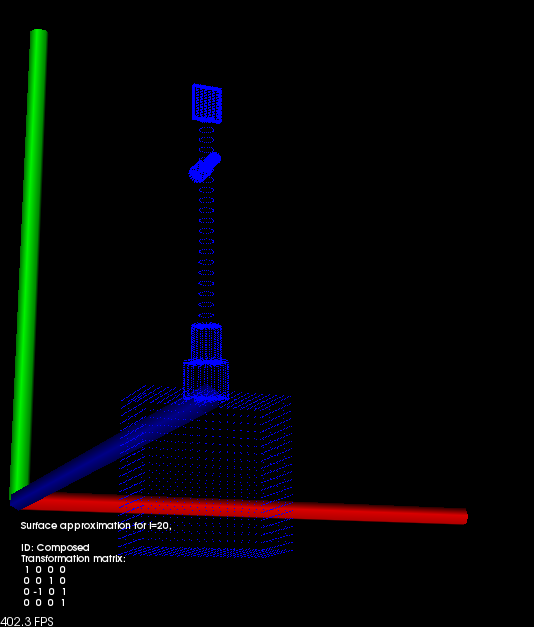
\includegraphics[height=3in]{./Results/Gripper_approx}
\caption{Gripper shape's approximation as a compound -- gripper's origin has
been moved away for visualization purposes}
\end{figure}


